\chapter{Multitask Learning using Semantic Relationship Data}

\section{Introduction}
In this chapter, we use machine learning to predict the compositionality of MWEs. We also add semantic role classification as an auxilliary task to see if our model can benefit from the shared learning and provide better predictions of compositionality. We find that training a model on both these tasks significantly improves its performance on each.

We start by introducing the datasets and methodology used in this study. We then perform experiments using single and multitask learning and discuss our results. Finally, we summarise our findings.
\section{Datasets}
In order to perform multitasking, we need both compositionality data and semantic relationship data. 
\subsection{Compositionality Datasets}
We reuse the datasets from \secref{sec:datasets}, combining \reddy, \ramisch and \discoj into a single dataset (referred to henceforth as \comp) with normalised compositionality scores ranging from 0 to 100.

We do not include \farahm in this consolidated dataset because its scores were on a binary scale. Although we are considering only the average of the scores for each MWE in \farahm, it is still not comparable to the other compositionality datasets that exhibit a range of compositionality scores. For example, \textit{water park} in \farahm was deemed compositional by half of the expert annotators and non-compositional by the other half and its average of 0.5 on a scale of 0 to 1 reflects this disagreement among annotators. However, a score of 50 out of 100 for any of the MWEs in \comp would imply it is semi-compositional, i.e. compositional with respect to one of its constituents. While this is true for most of the MWEs with an average of 0.5 in \farahm (and was indeed our motivation for considering the average of the scores), it may not always be the case. The average score of 0.5 is meant to convey that the MWE is equally likely to be compositional and non-compositional, based on inter-annotator agreement.

\noindent
We therefore have two compositionality datasets to experiment with in this chapter:
\begin{enumerate}
    \item \textbf{\comp} containing 325 binary MWES -- 180 compound nouns and 145 adjective-noun pairs with normalised overall compositionality scores ranging from 0 (completely non-compositional) to 100 (completely compositional).
    \item \textbf{\farahm} containing 1042 compound nouns and the average of their annotated compositionality scores ranginge [0,1].
\end{enumerate}

\subsection{Semantic Relationship Dataset}
The noun compound interpretation dataset from \cite{Tratz2010} contains 18,791 noun compounds with labels denoting one of 12 course semantic interpretations. For example, the NC \textit{campaign pledge} is assigned the label \textit{time} for its temporal significance while a \textit{marketing expert} is an expert in the topic of marketing and is therefore assigned the label \textit{topical}. There is also a fine-grained version of the dataset with 43 compound relations that build over the course-grained 12.

We use the course-grained dataset with 12 relations (see \tabref{tab:relations} for examples), which we refer to henceforth as \tratz.

\begin{table}[!htb]
\centering
\begin{tabular}{ll}
  \toprule
  Relation &\qquad Examples \\
  \midrule
  ATTRIBUTE &\qquad \textit{street name, earth tone} \\
  CAUSAL &\qquad \textit{court order, ad revenue} \\
  CAUSE &\qquad \textit{business interest, consumer taste} \\
  COMPLEMENT &\qquad \textit{fashion cycle, program clarity} \\
  CONTAINMENT &\qquad \textit{plastic bag, shoe box} \\
  LOC\_PART\_WHOLE &\qquad \textit{robot arm, hillside home} \\
  OBJECTIVE &\qquad \textit{finance director, poverty eradication} \\
  OWNER\_EMP\_USE &\qquad \textit{family estate, team doctor} \\
  PURPOSE &\qquad \textit{cooking pot, eye surgery} \\
  TIME &\qquad \textit{night work, birth date} \\
  TOPICAL &\qquad \textit{loan terms, job survey} \\
   \midrule
  OTHER &\qquad \textit{pig iron, contact lens} \\
\bottomrule
\end{tabular}
\caption{Course-grained relations in \tratz}
\label{tab:relations}
\end{table}

\begin{figure}[!htb]
\centering
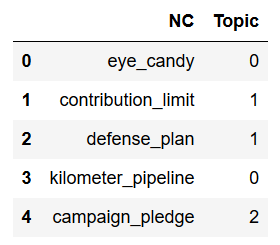
\includegraphics[width=.4\textwidth]{Figures/Tratz.PNG}
\caption{Semantic relationship data used in this study}
\end{figure}
\section{Methodology}
what are we trying to do? High-level
which is classification task so what is our output layer?
which is our regression task and what is the output?
\section{Experiments}
\begin{itemize}
    \item Gathering Data
    \item Preparing the Data -- \infersent embeddings, why \infersent?
    \item Choosing a Model -- keras framework, why keras? \\ Sequential model stacked layers, why sequential?
    \item Training -- 0.2 val split
    \item Evaluation -- 10-fold cross validation
    \item Hyperparameter Tuning -- dropout, nodes, number of hidden layers
    \item Prediction -- correlation scores for regression tasks, confusion matrix and accuracy for classification
\end{itemize}
\subsection{Single Task Learning}
\subsection{Multitask Learning}
multi-input multi-output model
\section{Results and Discussion}
\section{Summary}